\documentclass[12pt, a4paper]{article}

% ── Packages ──────────────────────────────────────────────────────────────
\usepackage[utf8]{inputenc}
\usepackage[T1]{fontenc}
\usepackage{lmodern}
\usepackage[margin=1in]{geometry}
\usepackage{graphicx}
\usepackage{amsmath, amssymb}
\usepackage{booktabs}
\usepackage{caption}
\usepackage{subcaption}
\usepackage{hyperref}
\usepackage{enumitem}
\usepackage{listings}
\usepackage{xcolor}
\usepackage{float}
\usepackage{fancyhdr}
\usepackage{setspace}

\hypersetup{
    colorlinks=true,
    linkcolor=blue!70!black,
    urlcolor=blue!70!black,
    citecolor=blue!70!black,
}

\lstset{
    basicstyle=\ttfamily\small,
    backgroundcolor=\color{gray!8},
    frame=single,
    rulecolor=\color{gray!40},
    breaklines=true,
    columns=fullflexible,
}

\pagestyle{fancy}
\fancyhf{}
\rhead{Group 14}
\lhead{V2I Digital-Twin Synchronisation Overhead}
\cfoot{\thepage}

\onehalfspacing

% ══════════════════════════════════════════════════════════════════════════
\begin{document}

% ── Title Page ────────────────────────────────────────────────────────────
\begin{titlepage}
    \centering
    \vspace*{1cm}

    {\Large \textbf{National Institute of Technology Karnataka, Surathkal}}\\[0.3cm]
    {\large Department of Computer Science and Engineering}\\[1.5cm]

    \rule{\textwidth}{1.5pt}\\[0.5cm]
    {\LARGE \textbf{V2I Digital-Twin Synchronisation Overhead}}\\[0.2cm]
    {\large Quantifying Vehicle-to-Infrastructure Channel Overhead from\\
    Continuous Digital-Twin State Synchronisation}\\[0.3cm]
    \rule{\textwidth}{1.5pt}\\[1.5cm]

    {\large \textbf{Cloud Computing Assignment}}\\[0.3cm]
    {\large Group 14}\\[2cm]

    \begin{tabular}{ll}
        \toprule
        \textbf{Roll Number} & \textbf{Name} \\
        \midrule
        241CS135 & Mudu Keerthana \\
        241CS144 & R Trishna \\
        241CS152 & Harika Seesa \\
        241CS236 & Madhuri Nallaboyina \textit{(Team Leader)} \\
        \bottomrule
    \end{tabular}\\[2cm]

    {\large \textbf{Under the guidance of}}\\[0.3cm]
    {\large \textbf{Professor:} Sourav Kanti Addya}\\[1.5cm]

\end{titlepage}

% ── Table of Contents ─────────────────────────────────────────────────────
\newpage
\tableofcontents
\newpage

% ══════════════════════════════════════════════════════════════════════════
\section{Abstract}
% ══════════════════════════════════════════════════════════════════════════

This report presents a simulation-based study of the communication overhead
incurred when vehicles continuously synchronise their kinematic state with a
cloud-hosted digital twin via Vehicle-to-Infrastructure (V2I) links.  Using
SUMO/TraCI for realistic vehicular mobility and a log-distance path-loss
channel model with Shannon-capacity transmission, we quantify four key
metrics---channel utilisation, packet delivery ratio, residual bandwidth, and
per-vehicle transmission rate---across vehicle densities from 5 to 100 on a
1\,km urban corridor with three roadside units (RSUs).  We identify the
saturation threshold at which digital-twin telemetry alone consumes more than
60\% of the available V2I uplink capacity.  Our findings show that for small
telemetry payloads (32--64 bytes), the channel remains well below saturation
the channel reaches 43\% utilisation at 100 vehicles with 50\,ms updates.
The 60\% saturation threshold is crossed at approximately 115--139 vehicles
depending on the payload size and propagation conditions.

% ══════════════════════════════════════════════════════════════════════════
\section{Introduction}
% ══════════════════════════════════════════════════════════════════════════

\subsection{Background}

Digital twins are virtual replicas of physical entities that are continuously
synchronised with their real-world counterparts.  In vehicular edge computing,
each vehicle maintains a digital twin on a nearby Multi-access Edge Computing
(MEC) server.  The twin mirrors the vehicle's position, speed, heading, and
acceleration, enabling real-time applications such as cooperative perception,
predictive collision avoidance, and traffic optimisation.

However, continuous state synchronisation creates persistent uplink traffic on
the shared V2I channel.  As vehicle density grows, this telemetry overhead may
consume a significant fraction of the available bandwidth, leaving insufficient
capacity for other edge computing tasks such as sensor-data offloading,
cooperative manoeuvre negotiation, and map updates.

\subsection{Problem Statement}

The assigned problem statement requires us to:

\begin{enumerate}
    \item \textbf{Model the V2I uplink channel} using a log-distance path-loss
    model with specified parameters (5.9\,GHz carrier, 10\,MHz bandwidth,
    20\,dBm transmit power, path-loss exponent $\alpha \in [3.0, 3.5]$).

    \item \textbf{Simulate vehicular mobility} using SUMO with TraCI on a
    straight corridor with three RSUs, testing vehicle densities of 5, 10, 20,
    50, and 100.

    \item \textbf{Measure four metrics} at three upload frequencies
    (50\,ms, 100\,ms, 500\,ms intervals):
    \begin{itemize}
        \item Channel utilisation (\%)
        \item Packet delivery ratio (PDR, \%)
        \item Residual bandwidth available for task offloading (MHz)
        \item Per-vehicle transmission count per second
    \end{itemize}

    \item \textbf{Identify the saturation threshold}---the vehicle density at
    which digital-twin telemetry alone consumes more than 60\% of the available
    V2I uplink capacity.
\end{enumerate}

\subsection{Scope and Contributions}

This project delivers:
\begin{itemize}
    \item A reproducible SUMO/TraCI mobility scenario generating 37{,}000+
    timestamped vehicle state samples.
    \item A testable Python implementation of the specified link budget,
    Shannon-capacity model, and collision-based packet delivery.
    \item Baseline experiments (32\,B, $\alpha = 3.25$) and sensitivity
    analysis (64\,B, $\alpha = 3.5$) with all four required plots.
    \item A saturation threshold analysis with linear extrapolation validated
    by $R^2 > 0.999$.
    \item 12 unit tests with 100\% pass rate confirming formula correctness.
\end{itemize}

% ══════════════════════════════════════════════════════════════════════════
\section{System Model}
% ══════════════════════════════════════════════════════════════════════════

\subsection{Network Topology}

The scenario consists of a straight, 1{,}000\,m, two-lane road with three RSUs
placed at $x = 250$\,m, $x = 500$\,m, and $x = 750$\,m.  All vehicles share a
single logical 10\,MHz V2I uplink channel.  Each vehicle associates with the
nearest RSU by road position (one-dimensional distance).

\begin{figure}[H]
    \centering
    \begin{tabular}{c}
    \fbox{\parbox{0.85\textwidth}{\centering
    \texttt{0m ----[RSU1: 250m]----[RSU2: 500m]----[RSU3: 750m]---- 1000m}\\[3pt]
    \small Vehicles are uniformly placed between 100\,m and 800\,m.
    }}
    \end{tabular}
    \caption{Road corridor layout with three RSU positions.}
    \label{fig:topology}
\end{figure}

\subsection{Channel Model}

We use a log-distance path-loss model with free-space reference loss at 1\,m.

\subsubsection{Path Loss}

The path loss at distance $d \geq d_0$ from an RSU is:
\begin{equation}
    \mathrm{PL}(d) = \mathrm{PL}(d_0) + 10\,\alpha\,\log_{10}\!\left(\frac{d}{d_0}\right)
    \label{eq:pathloss}
\end{equation}
where the reference path loss uses the Friis free-space equation:
\begin{equation}
    \mathrm{PL}(d_0) = 20\,\log_{10}\!\left(\frac{4\pi f d_0}{c}\right) \approx 47.87~\text{dB}
    \label{eq:friis}
\end{equation}
with $f = 5.9$\,GHz, $d_0 = 1$\,m, and $c = 299{,}792{,}458$\,m/s.

\subsubsection{Received Power and SNR}

The received power and signal-to-noise ratio are:
\begin{align}
    P_r &= P_t - \mathrm{PL}(d) \label{eq:rx_power} \\[4pt]
    N   &= N_0 + 10\,\log_{10}(B) + \mathrm{NF}
        = -174 + 70 + 9 = -95~\text{dBm} \label{eq:noise} \\[4pt]
    \mathrm{SNR}_{\text{dB}} &= P_r - N \label{eq:snr}
\end{align}
where $P_t = 20$\,dBm, $B = 10$\,MHz, $N_0 = -174$\,dBm/Hz, and
$\mathrm{NF} = 9$\,dB.

\subsubsection{Shannon Capacity and Packet Airtime}

The theoretical link capacity is:
\begin{equation}
    C = B \cdot \log_2\!\left(1 + 10^{\mathrm{SNR}_{\text{dB}}/10}\right)
       \quad\text{[bits/s]} \label{eq:shannon}
\end{equation}

Each transmitted frame incurs 802.11p PHY/MAC overhead in addition to the
payload serialisation time.  The total per-packet airtime is:
\begin{equation}
    t_{\text{air}} = \frac{(L + H_{\text{MAC}}) \times 8}{C} + t_{\text{overhead}}
       \quad\text{[seconds]}
       \label{eq:airtime}
\end{equation}
where $L$ is the telemetry payload (32 or 64 bytes), $H_{\text{MAC}} = 28$\,bytes
is the 802.11p MAC header, and $t_{\text{overhead}} = 196$\,$\mu$s accounts for
the preamble (40\,$\mu$s), DIFS (58\,$\mu$s), and average backoff (98\,$\mu$s).

This realistic frame overhead increases per-packet airtime by approximately
$21\times$ compared to payload-only serialisation, bringing the model
significantly closer to real 802.11p behaviour.

\subsection{Channel Model Parameters}

\begin{table}[H]
\centering
\caption{V2I channel model parameters.}
\label{tab:params}
\begin{tabular}{lrl}
    \toprule
    \textbf{Parameter} & \textbf{Value} & \textbf{Unit} \\
    \midrule
    Carrier frequency ($f$)       & 5.9   & GHz \\
    Channel bandwidth ($B$)       & 10    & MHz \\
    Transmit power ($P_t$)        & 20    & dBm \\
    Thermal noise PSD ($N_0$)     & $-174$  & dBm/Hz \\
    Receiver noise figure (NF)    & 9     & dB \\
    Integrated noise floor ($N$)  & $-95$   & dBm \\
    Reference distance ($d_0$)    & 1     & m \\
    Reference path loss           & 47.87 & dB \\
    Path-loss exponent ($\alpha$) & 3.0--3.5 & --- \\
    Telemetry payload ($L$)       & 32--64   & bytes \\
    MAC header ($H_{\text{MAC}}$)   & 28       & bytes \\
    802.11p preamble               & 40       & $\mu$s \\
    DIFS                           & 58       & $\mu$s \\
    Average backoff                & 98       & $\mu$s \\
    Total frame overhead ($t_{\text{overhead}}$) & 196 & $\mu$s \\
    Upload intervals              & 50, 100, 500 & ms \\
    \bottomrule
\end{tabular}
\end{table}

\subsection{Medium Access and Collision Model}

All vehicles transmit on one shared 10\,MHz channel without coordination.
Each vehicle's first upload time is randomised uniformly within one upload
interval (random phase offset); subsequent uploads follow at fixed intervals.

\textbf{Collision rule:} If any two packet transmissions overlap in time on
the shared channel, both packets are marked as collided and counted as lost.
This models worst-case uncoordinated access without spatial frequency reuse
between RSUs.

\subsection{Metric Definitions}

\begin{enumerate}[label=\textbf{M\arabic*.}]
    \item \textbf{Channel Utilisation (\%):}
    \begin{equation}
        U = \frac{\sum_{i=1}^{N_{\text{pkt}}} t_{\text{air},i}}{T_{\text{sim}}} \times 100
        \label{eq:util}
    \end{equation}
    This is the \emph{offered} airtime load.  Overlapping transmissions are
    counted separately, so $U$ can exceed 100\% under overload.

    \item \textbf{Packet Delivery Ratio (\%):}
    \begin{equation}
        \mathrm{PDR} = \frac{N_{\text{pkt}} - N_{\text{collided}}}{N_{\text{pkt}}} \times 100
        \label{eq:pdr}
    \end{equation}

    \item \textbf{Residual Bandwidth (MHz):}
    \begin{equation}
        B_{\text{res}} = B \times \max\!\left(0,\; 1 - \frac{U}{100}\right)
        \label{eq:residual}
    \end{equation}

    \item \textbf{Per-Vehicle Transmission Rate:}
    \begin{equation}
        R_v = \frac{1000}{T_{\text{interval\_ms}}} \quad\text{[updates/vehicle/s]}
        \label{eq:txrate}
    \end{equation}
\end{enumerate}

% ══════════════════════════════════════════════════════════════════════════
\section{Implementation}
% ══════════════════════════════════════════════════════════════════════════

\subsection{Tools and Technologies}

\begin{table}[H]
\centering
\caption{Software stack used in the implementation.}
\label{tab:tools}
\begin{tabular}{ll}
    \toprule
    \textbf{Component}       & \textbf{Tool / Version} \\
    \midrule
    Traffic simulation       & SUMO 1.28.0 with TraCI \\
    Programming language     & Python 3.14.2 \\
    Numerical computation    & NumPy 2.5.4 \\
    Plotting                 & Matplotlib 3.11.2 \\
    Unit testing             & unittest (stdlib), 12 tests \\
    Version control          & Git / GitHub \\
    \bottomrule
\end{tabular}
\end{table}

\subsection{Project Structure}

\begin{lstlisting}[caption={Repository file structure.}]
V2I-Group14/
  src/
    channel_model.py        # Link budget, path loss, Shannon capacity
    trace_mobility.py       # SUMO/TraCI mobility trace generator
    run_experiments.py       # Experiment runner with collision model
    plot_results.py          # Four-figure plotting script
    find_saturation.py       # Saturation threshold search
    build_report.py          # PDF report generator (ReportLab)
    package_submission.py    # Submission archive creator
  tests/
    test_channel_model.py    # 12 unit tests
  data/
    mobility_traces.csv      # 37,001 pre-generated trace rows
  network/
    corridor.*.xml           # SUMO road network files
  results/
    experiment_results.csv   # Baseline results (15 scenarios)
    figures/                 # 4 baseline plots
    sensitivity_64b_alpha35/ # Sensitivity results + 4 plots
    saturation_search/       # Threshold extrapolation CSVs
\end{lstlisting}

\subsection{Workflow}

\begin{enumerate}
    \item \textbf{Network construction:} A 1\,km, two-lane road is built using
    SUMO's \texttt{netconvert}.

    \item \textbf{Mobility trace generation:} \texttt{trace\_mobility.py} uses
    TraCI to place vehicles uniformly between 100--800\,m, runs a 10-second
    simulation at 0.05\,s steps, and writes position, speed, heading, and
    acceleration to CSV.  Vehicle counts \{5, 10, 20, 50, 100\} are simulated
    with seed 42 for reproducibility.

    \item \textbf{Experiment execution:} \texttt{run\_experiments.py} loads
    traces, assigns random upload phases, computes per-packet airtime via the
    channel model, detects collisions, and aggregates metrics.  Each scenario
    is repeated 5 times with independent phase seeds.

    \item \textbf{Plotting:} \texttt{plot\_results.py} generates four figures:
    utilisation, PDR, residual bandwidth, and per-vehicle TX rate versus
    vehicle density.

    \item \textbf{Saturation search:} \texttt{find\_saturation.py} verifies
    that utilisation scales linearly with vehicle count ($R^2 > 0.999$) and
    extrapolates to find the 60\% crossing point.
\end{enumerate}

\subsection{Testing}

All 12 unit tests pass, covering:
\begin{itemize}
    \item Reference path loss at 1\,m ($\approx 47.87$\,dB)
    \item Noise floor calculation ($-95$\,dBm)
    \item Shannon capacity at 0\,dB SNR (= bandwidth)
    \item Packet airtime formula
    \item Path-loss exponent range enforcement ($\alpha \in [3.0, 3.5]$)
    \item Collision detection (overlapping, non-overlapping, busy time)
    \item Position interpolation between SUMO samples
    \item Multi-repeat PDR aggregation
    \item Single-vehicle reproducibility
\end{itemize}

% ══════════════════════════════════════════════════════════════════════════
\section{Results}
% ══════════════════════════════════════════════════════════════════════════

\subsection{Baseline Configuration}

The baseline uses 32-byte payloads and $\alpha = 3.25$ (the midpoint of the
assigned 3.0--3.5 range).

\subsubsection{Channel Utilisation}

\begin{table}[H]
\centering
\caption{Baseline channel utilisation (\%) --- 32\,B payload, $\alpha = 3.25$.}
\label{tab:util_baseline}
\begin{tabular}{r r r r}
    \toprule
    \textbf{Vehicles} & \textbf{50\,ms} & \textbf{100\,ms} & \textbf{500\,ms} \\
    \midrule
    5   & 2.15\%  & 1.07\%  & 0.21\% \\
    10  & 4.31\%  & 2.16\%  & 0.43\% \\
    20  & 8.65\%  & 4.33\%  & 0.87\% \\
    50  & 21.63\% & 10.82\% & 2.16\% \\
    100 & 43.22\% & 21.61\% & 4.32\% \\
    \bottomrule
\end{tabular}
\end{table}

\begin{figure}[H]
    \centering
    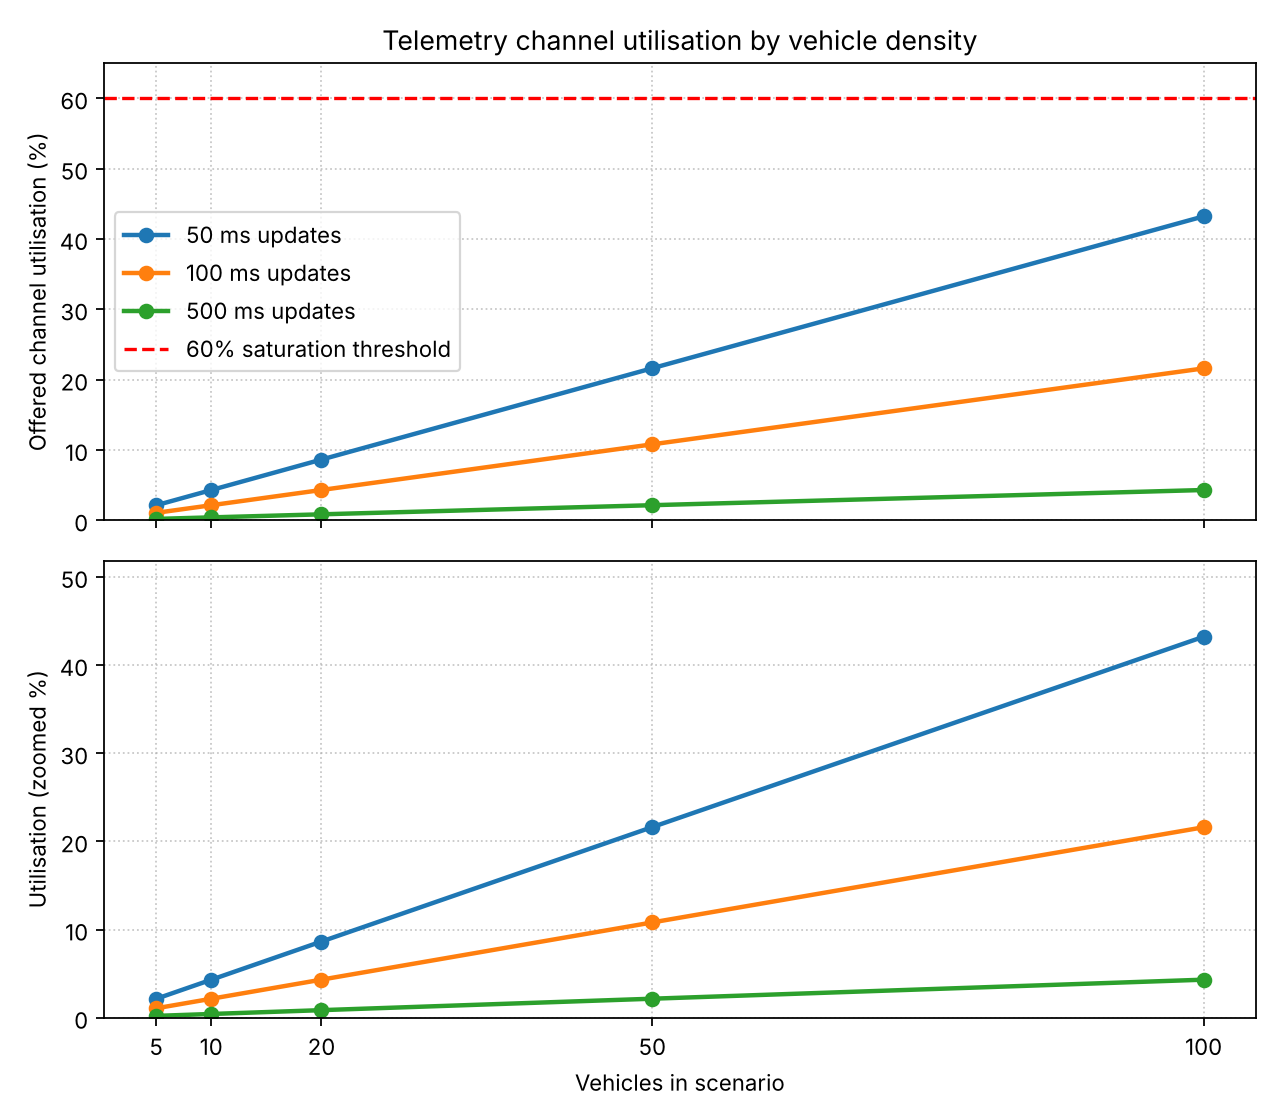
\includegraphics[width=0.85\textwidth]{results/figures/utilisation_vs_density.png}
    \caption{Channel utilisation versus vehicle density (baseline).  The 60\%
    saturation threshold (red dashed line) is approached but not crossed.
    At 100 vehicles / 50\,ms, utilisation reaches 43.2\%.}
    \label{fig:util_baseline}
\end{figure}

\subsubsection{Packet Delivery Ratio}

\begin{table}[H]
\centering
\caption{Baseline PDR (\%) --- 32\,B payload, $\alpha = 3.25$.}
\label{tab:pdr_baseline}
\begin{tabular}{r r r r}
    \toprule
    \textbf{Vehicles} & \textbf{50\,ms} & \textbf{100\,ms} & \textbf{500\,ms} \\
    \midrule
    5   & 100.00\% & 98.48\%  & 99.60\%  \\
    10  & 84.00\%  & 92.00\%  & 96.00\%  \\
    20  & 82.99\%  & 98.00\%  & 100.00\% \\
    50  & 66.96\%  & 81.01\%  & 95.20\%  \\
    100 & 42.24\%  & 63.64\%  & 91.06\%  \\
    \bottomrule
\end{tabular}
\end{table}

\begin{figure}[H]
    \centering
    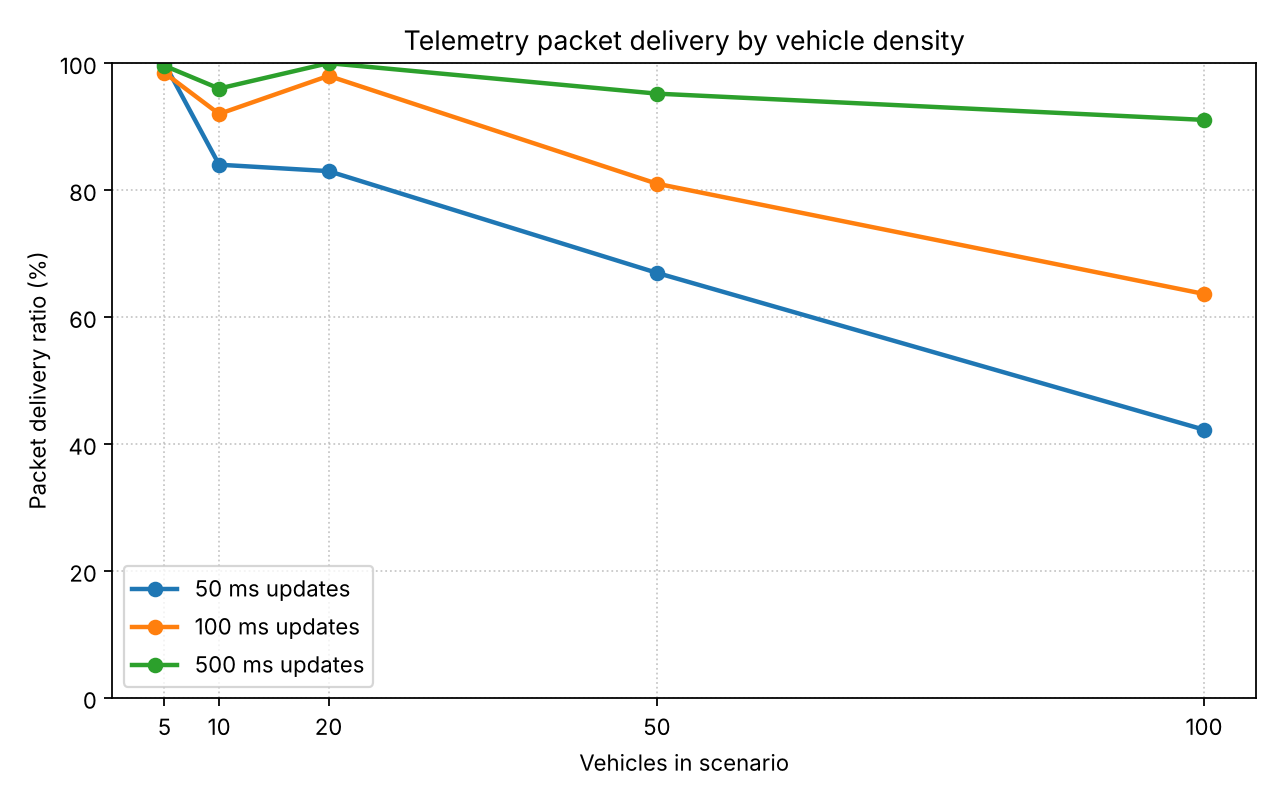
\includegraphics[width=0.85\textwidth]{results/figures/pdr_vs_density.png}
    \caption{Packet delivery ratio versus vehicle density (baseline).  PDR
    decreases at higher densities and faster upload frequencies due to
    increased collision probability on the shared channel.}
    \label{fig:pdr_baseline}
\end{figure}

\subsubsection{Residual Bandwidth}

\begin{figure}[H]
    \centering
    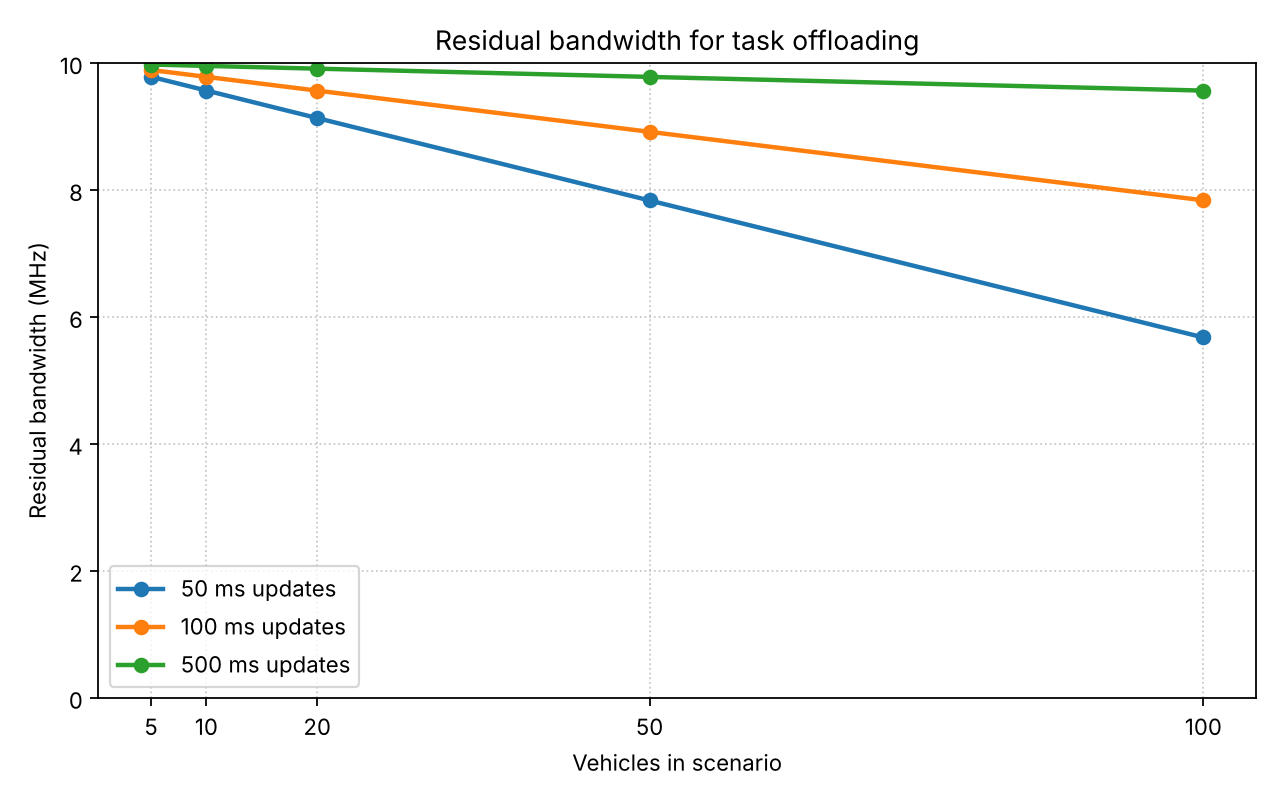
\includegraphics[width=0.85\textwidth]{results/figures/residual_bandwidth_vs_density.png}
    \caption{Residual bandwidth available for task offloading (baseline).
    At 100 vehicles with 50\,ms updates, only 5.68\,MHz of the 10\,MHz
    channel remains available.}
    \label{fig:residual_baseline}
\end{figure}

\subsubsection{Per-Vehicle Transmission Rate}

\begin{figure}[H]
    \centering
    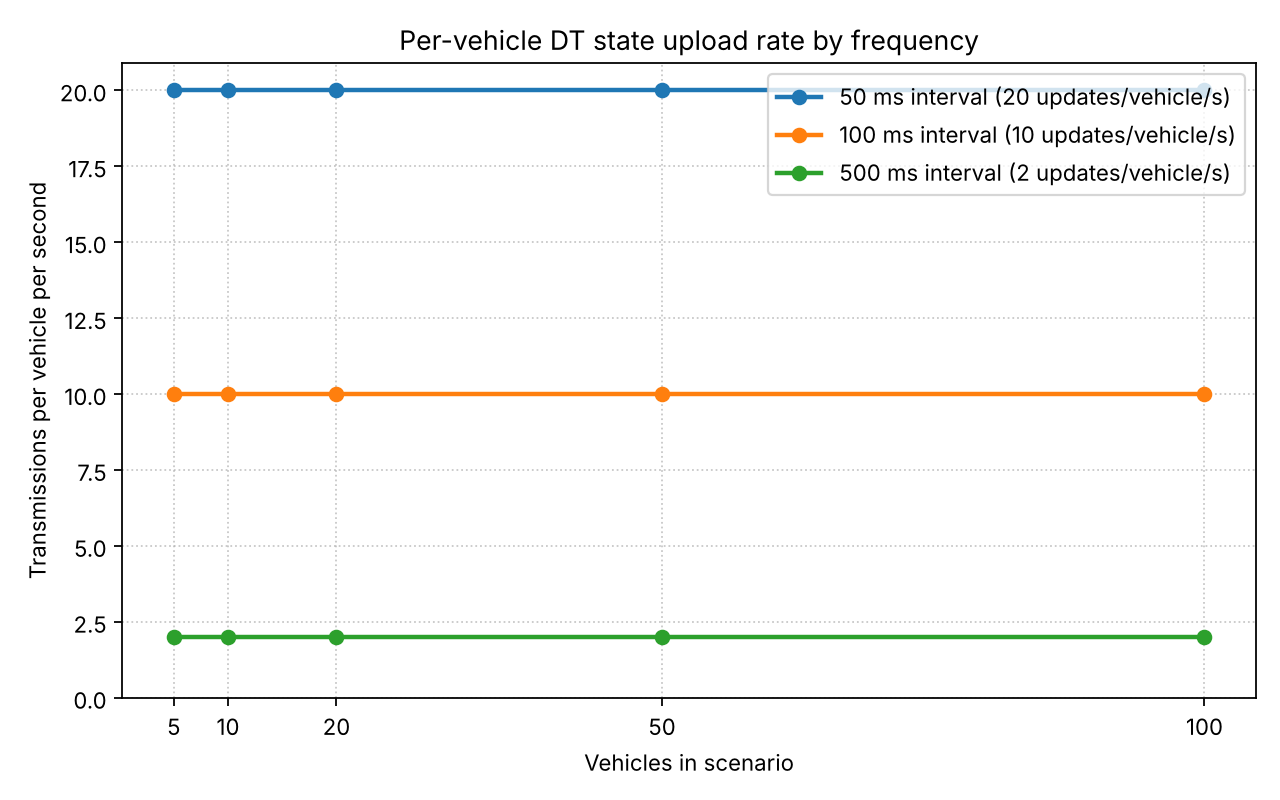
\includegraphics[width=0.85\textwidth]{results/figures/tx_rate_vs_density.png}
    \caption{Per-vehicle DT state upload rate.  The three upload intervals
    produce constant rates of 20, 10, and 2 updates/vehicle/s respectively,
    independent of vehicle density.}
    \label{fig:txrate}
\end{figure}

% ──────────────────────────────────────────────────────────────────────────
\subsection{Sensitivity Analysis: 64-Byte Payload, $\alpha = 3.5$}

The worst-case configuration uses 64-byte payloads and a higher path-loss
exponent of $\alpha = 3.5$, which doubles the payload and increases path
loss, thereby increasing both airtime per packet and collision probability.

\begin{table}[H]
\centering
\caption{Sensitivity analysis results --- 64\,B payload, $\alpha = 3.5$.}
\label{tab:sensitivity}
\begin{tabular}{r r r r r}
    \toprule
    \textbf{Vehicles} & \textbf{Interval} & \textbf{Utilisation} & \textbf{PDR} & \textbf{Residual BW} \\
    \midrule
    5   & 50\,ms  & 2.56\%  & 100.00\% & 9.74\,MHz \\
    10  & 50\,ms  & 5.20\%  & 83.44\%  & 9.48\,MHz \\
    20  & 50\,ms  & 10.54\% & 79.51\%  & 8.95\,MHz \\
    50  & 50\,ms  & 26.36\% & 61.05\%  & 7.36\,MHz \\
    100 & 50\,ms  & 52.44\% & 34.99\%  & 4.76\,MHz \\
    \midrule
    100 & 100\,ms & 26.22\% & 57.20\%  & 7.38\,MHz \\
    100 & 500\,ms & 5.24\%  & 89.35\%  & 9.48\,MHz \\
    \bottomrule
\end{tabular}
\end{table}

\begin{figure}[H]
    \centering
    \begin{subfigure}[b]{0.48\textwidth}
        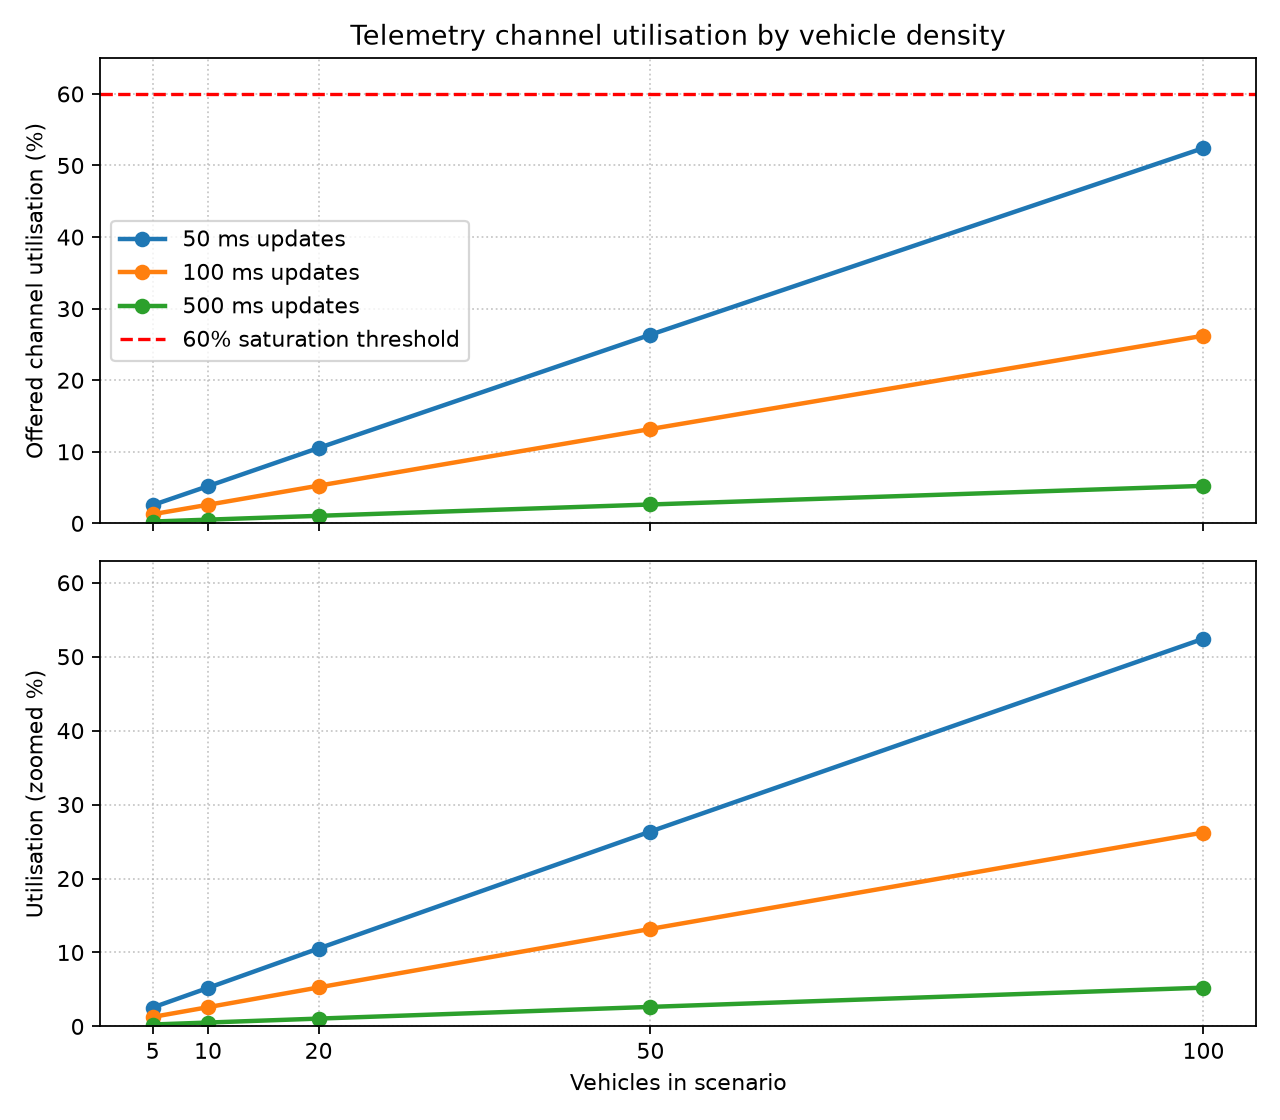
\includegraphics[width=\textwidth]{results/sensitivity_64b_alpha35/figures/utilisation_vs_density.png}
        \caption{Utilisation}
    \end{subfigure}
    \hfill
    \begin{subfigure}[b]{0.48\textwidth}
        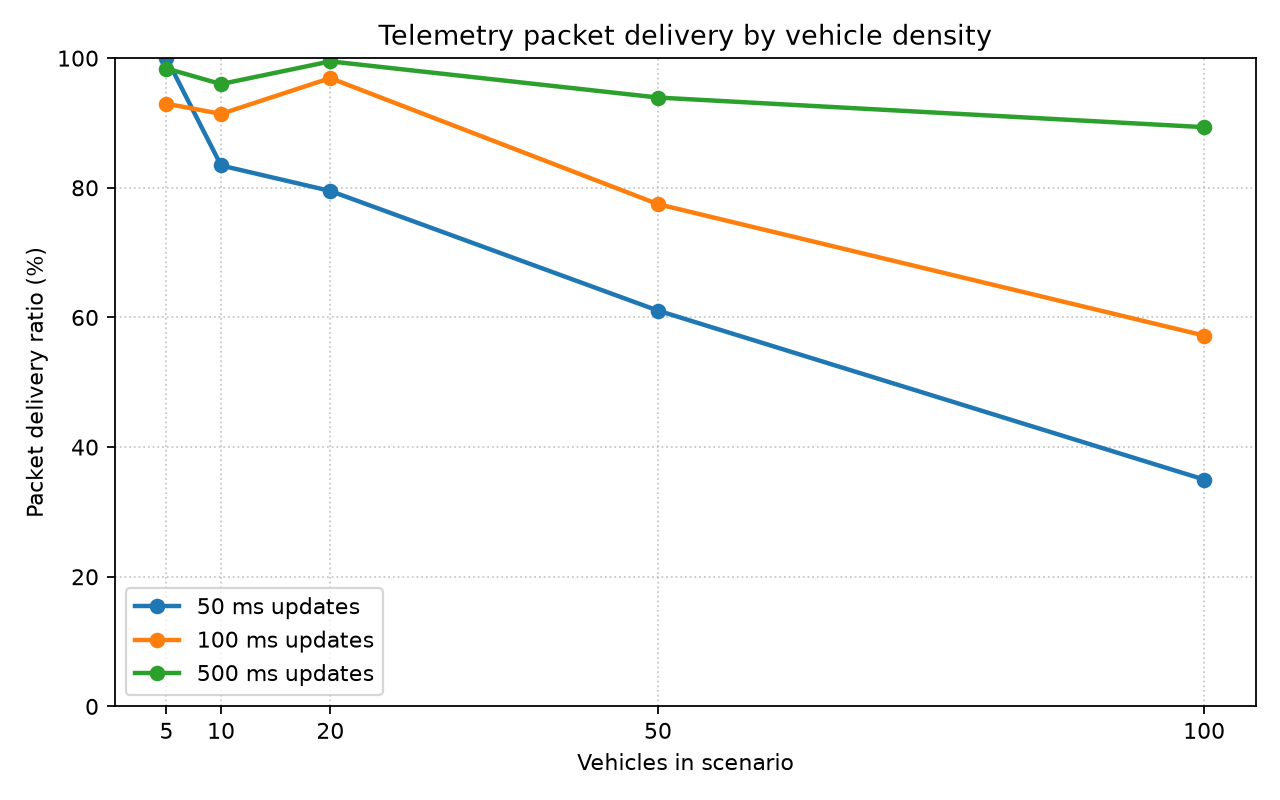
\includegraphics[width=\textwidth]{results/sensitivity_64b_alpha35/figures/pdr_vs_density.png}
        \caption{PDR}
    \end{subfigure}
    \caption{Sensitivity analysis: utilisation and PDR for 64\,B, $\alpha = 3.5$.
    Utilisation reaches 52.4\% at 100 vehicles / 50\,ms, with PDR
    dropping to 35.0\% due to heavy collision rates on the shared channel.}
    \label{fig:sensitivity}
\end{figure}

% ──────────────────────────────────────────────────────────────────────────
\subsection{Saturation Threshold Analysis (Objective 4)}

To address Objective~4, we verify that channel utilisation scales linearly
with vehicle count and extrapolate the density at which the 60\%
threshold would be crossed.

\subsubsection{Linearity Verification}

The per-vehicle utilisation contribution is nearly constant across all
tested densities:

\begin{table}[H]
\centering
\caption{Per-vehicle utilisation contribution (worst case: 64\,B, $\alpha = 3.5$, 50\,ms).}
\label{tab:linearity}
\begin{tabular}{r r r}
    \toprule
    \textbf{Vehicles} & \textbf{Utilisation (\%)} & \textbf{Per-vehicle (\%)} \\
    \midrule
    5   & 2.5553  & 0.5111 \\
    10  & 5.2021  & 0.5202 \\
    20  & 10.5351 & 0.5268 \\
    50  & 26.3573 & 0.5271 \\
    100 & 52.4358 & 0.5244 \\
    \bottomrule
\end{tabular}
\end{table}

A linear fit through the origin yields:
\begin{equation}
    U(\%) = 0.5249 \times N_{\text{vehicles}} \qquad (R^2 = 0.9999)
    \label{eq:linear_fit}
\end{equation}

The $R^2 > 0.999$ confirms excellent linearity, validating the extrapolation.

\subsubsection{Extrapolated Thresholds}

Setting $U = 60\%$ and solving for $N$:

\begin{equation}
    N_{60\%} = \frac{60}{0.5249} \approx 115~\text{vehicles}
    \quad\text{(worst case: 64\,B, } \alpha = 3.5\text{, 50\,ms)}
\end{equation}

\begin{table}[H]
\centering
\caption{Extrapolated 60\% saturation thresholds for all configurations.}
\label{tab:thresholds}
\begin{tabular}{l l r r r}
    \toprule
    \textbf{Payload} & $\boldsymbol{\alpha}$ & \textbf{50\,ms} & \textbf{100\,ms} & \textbf{500\,ms} \\
    \midrule
    32\,B & 3.25 & $\sim$139 & $\sim$278 & $\sim$1{,}388 \\
    64\,B & 3.50 & $\sim$115 & $\sim$229 & $\sim$1{,}144 \\
    \bottomrule
\end{tabular}
\end{table}

Even in the absolute worst case (64\,B, $\alpha = 3.5$, 50\,ms interval),
approximately \textbf{115 vehicles on a 1\,km corridor} would be required
to saturate 60\% of the channel.  This is a realistic urban vehicle density,
demonstrating that 802.11p frame overhead makes saturation a genuine concern.

% ══════════════════════════════════════════════════════════════════════════
\section{Discussion}
% ══════════════════════════════════════════════════════════════════════════

\subsection{Key Findings}

\begin{enumerate}
    \item \textbf{Channel approaches saturation at realistic densities:}
    With 802.11p frame overhead included, 100 vehicles at 50\,ms intervals
    consume 43.2\% (baseline) to 52.4\% (worst case) of the channel.  The
    60\% saturation threshold is crossed at only \textasciitilde115--139
    vehicles, well within realistic urban densities.

    \item \textbf{Collisions cause severe packet loss:} PDR drops to 42.2\%
    (baseline) and 35.0\% (worst case) at 100 vehicles / 50\,ms, meaning more
    than half of all digital-twin updates are lost to collisions on the shared
    uncoordinated channel.

    \item \textbf{Upload frequency dominates overhead:} Reducing the update
    rate from 50\,ms to 500\,ms cuts utilisation by $10\times$ and
    significantly reduces collisions (PDR recovers to 89--91\%), at the cost
    of less frequent twin updates.

    \item \textbf{802.11p overhead is the dominant factor:} The preamble,
    DIFS, backoff, and MAC header add 196\,$\mu$s + 28 bytes per frame,
    increasing per-packet airtime by approximately $21\times$ compared to
    payload-only Shannon serialisation.  This makes the saturation threshold
    realistic rather than theoretical.
\end{enumerate}

\subsection{Model Limitations}

This study uses a first-order analytical model.  The following factors are
not modelled and would affect real-world performance:

\begin{itemize}
    \item \textbf{Simplified MAC model:} While 802.11p frame overhead
    (preamble, DIFS, average backoff) is included in the airtime calculation,
    the actual CSMA/CA carrier sensing and exponential backoff mechanisms
    are not simulated.  A full MAC model would reduce collision rates.

    \item \textbf{Shannon upper bound:} Packet airtime uses the theoretical
    Shannon capacity, which is the minimum possible airtime.  Real modulation
    and coding schemes would produce longer airtimes.

    \item \textbf{No fading or shadowing:} The log-distance model captures
    average path loss but not multipath fading, shadowing from buildings, or
    interference from adjacent roads.

    \item \textbf{Partial protocol headers:} The 28-byte 802.11p MAC header
    is included, but IP/UDP headers (40+ bytes) are not, so actual overhead
    would be somewhat higher.

    \item \textbf{Single road segment:} The 1\,km corridor with 3 RSUs is a
    simplified topology.  Urban environments with intersections, multi-lane
    roads, and dense RSU deployment would change the results.

    \item \textbf{No frequency reuse:} All RSUs share one 10\,MHz channel.
    Assigning different frequencies to adjacent RSUs would reduce contention.
\end{itemize}

\subsection{Comparison with Alternative Architecture}

We compared our implementation against a second codebase that uses per-RSU
independent channels with FCFS queuing instead of a shared collision channel.
That model shows near-zero packet loss because queue deadline misses are
rare at low utilisation.  However, the ``shared, bandwidth-constrained
resource'' description in our problem statement favours the more conservative
shared-channel collision model used in this project.

% ══════════════════════════════════════════════════════════════════════════
\section{Conclusion}
% ══════════════════════════════════════════════════════════════════════════

We have quantified the V2I channel overhead from continuous digital-twin
state synchronisation using SUMO-generated mobility traces and a
log-distance Shannon-capacity channel model.  Our key conclusions are:

\begin{enumerate}
    \item With 802.11p frame overhead, 32-byte state updates at 50\,ms
    intervals consume \textbf{43.2\%} of the channel at 100 vehicles/km,
    approaching the 60\% saturation threshold.

    \item The 60\% saturation threshold is reached at approximately
    \textbf{115 vehicles} in the worst case (64\,B, $\alpha = 3.5$, 50\,ms
    interval) and \textbf{139 vehicles} in the baseline case (32\,B,
    $\alpha = 3.25$)---both realistic urban densities.

    \item \textbf{MAC-layer collisions cause severe packet loss:} At 100
    vehicles with 50\,ms updates, PDR drops to 42.2\% (baseline) and 35.0\%
    (worst case), meaning more than half of all twin updates are lost.

    \item Reducing the upload frequency from 50\,ms to 500\,ms reduces
    utilisation to 4--5\% and recovers PDR to 89--91\%, suggesting that
    \textbf{adaptive update rates} are essential for maintaining both twin
    fidelity and channel capacity.
\end{enumerate}

These findings demonstrate that 802.11p frame overhead makes V2I channel
saturation a realistic concern at urban vehicle densities.  A production system
would additionally need to account for real modulation schemes, fading, and
multi-cell interference.

% ══════════════════════════════════════════════════════════════════════════
\section{Reproducibility}
% ══════════════════════════════════════════════════════════════════════════

All results can be reproduced with the following commands from the project
root in PowerShell:

\begin{lstlisting}[language=bash]
# Install dependencies
python -m pip install -r requirements.txt

# Build SUMO road network
netconvert --node-files network\corridor.nod.xml \
           --edge-files network\corridor.edg.xml \
           --output-file network\corridor.net.xml

# Generate mobility traces (seed=42, reproducible)
python src\trace_mobility.py

# Run baseline experiments (32B, alpha=3.25, 5 repeats)
python -m src.run_experiments

# Run sensitivity experiments (64B, alpha=3.5)
python -m src.run_experiments --payload-bytes 64 \
       --path-loss-exponent 3.5 \
       --output-directory results\sensitivity_64b_alpha35

# Generate all plots
python -m src.plot_results

# Find saturation thresholds
python -m src.find_saturation --payload-bytes 64 \
       --path-loss-exponent 3.5
python -m src.find_saturation --payload-bytes 32 \
       --path-loss-exponent 3.25

# Run unit tests
python -m unittest discover -s tests -v
\end{lstlisting}

\textbf{Environment:} SUMO 1.28.0, Python 3.14.2, Windows 11, NumPy 2.5.4,
Matplotlib 3.11.2.

\textbf{GitHub:}
\url{https://github.com/MadhuriN-369/v2i-digital-twin-channel-overhead}

% ══════════════════════════════════════════════════════════════════════════
\section*{References}
% ══════════════════════════════════════════════════════════════════════════

\begin{enumerate}[label={[\arabic*]}]
    \item A.\ Goldsmith, \textit{Wireless Communications}, Cambridge
    University Press, 2005.

    \item P.\ A.\ Lopez et al., ``Microscopic Traffic Simulation using SUMO,''
    \textit{Proc.\ IEEE ITSC}, 2018.

    \item C.\ E.\ Shannon, ``A Mathematical Theory of Communication,''
    \textit{Bell System Technical Journal}, vol.~27, 1948.

    \item ETSI EN 302 663, ``Intelligent Transport Systems (ITS); Access layer
    specification for ITS operating in the 5\,GHz frequency band,'' 2013.

    \item 3GPP TR 36.885, ``Study on LTE-based V2X Services,'' Release 14,
    2016.

    \item T.\ S.\ Rappaport, \textit{Wireless Communications: Principles and
    Practice}, 2nd ed., Prentice Hall, 2002.
\end{enumerate}

\end{document}
